\documentclass[12pt]{article}
\usepackage{../preamble2}

\title{A Grid Number Puzzle}
\author{https://puzzling.stackexchange.com/questions/99712/almost-impossible-sudoku-like-puzzle}
\date{8 July 2020}

\begin{document}

\begin{question}

Place the first eight positive integers in the grid below such that sums along blocks of three squares are equal.
\begin{center}
  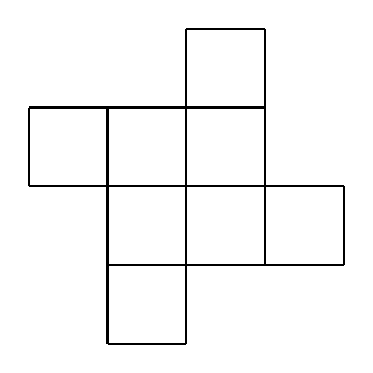
\begin{tikzpicture}
    \draw[help lines, black, thick] (0,0) grid (1,1) (1,-2) grid (2,1) (2,-1) grid (3,2) (3,-1) grid (4,0);
  \end{tikzpicture}
\end{center}

\end{question}
For convenience, label the boxes with letters:
\begin{center}
  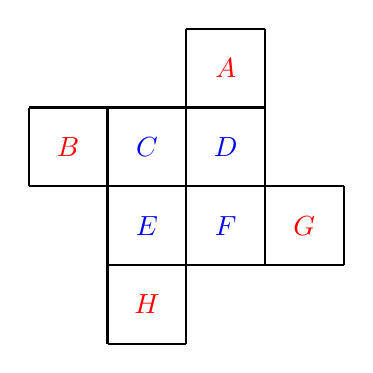
\begin{tikzpicture}
    \draw[help lines, black, thick] (0,0) grid (1,1) (1,-2) grid (2,1) (2,-1) grid (3,2) (3,-1) grid (4,0);
    \node [red] at (2.5,1.5) {$A$};
    \node [red] at (0.5,0.5) {$B$};
    \node [blue] at (1.5,0.5) {$C$};
    \node [blue] at (2.5,0.5) {$D$};
    \node [blue] at (1.5,-0.5) {$E$};
    \node [blue] at (2.5,-0.5) {$F$};
    \node [red] at (3.5,-0.5) {$G$};
    \node [red] at (1.5,-1.5) {$H$};
  \end{tikzpicture}
\end{center}
First note that the grid can be rotated four ways: $A\longrightarrow G$, $A\longrightarrow H$, $A\longrightarrow B$. Thus by symmetry, there are $4$ equivalent arrangement of numbers. 

There are $48$ permutations that keep the row-sums and column-sums constant. We divide by $4$ to remove solutions that are obtained by rotation. We are therefore looking for $12$ distinct solutions! 

Let $S$ denote the sum along blocks of three. 
\begin{align*}
S & = B + C + D\\
  & = E + F + G\\
  & = C + E + H\\
  & = A + D + F\\
\end{align*} 
Let $M$ denote the sum of the middle four squares (the blue squares).
\begin{align*}
M = C + D + E + F
\end{align*} 
Adding the sums gives
\begin{align*}
4S = A + B + C + D + E + F + G + H + M
\end{align*}
We also have 
\begin{align*}
A + B + C + D + E + F + G + H = 1 + 2 + \ldots + 7 + 8 = \frac{8 \times 9}{2} = 36
\end{align*}
Combining these, we get
\begin{align*}
4S & = 36 + M \\
 M & = 4(S-9)
\end{align*} 
$M$ must be a multiple of $4$. Moreover, the lowest possible value for $M$ is $1+2+3+4=10$, and the highest possible value is $8+7+6+5=26$. This gives possible values for $M$ of $12$, $16$, $20$, $24$. To these correspond possible values of $S$ of $9+M/4=$ $12$, $13$, $14$, $15$.

\textbf{Consider $\mathbf{S=15~(M=24)}$}. Since $8+7=15$, the middle squares cannot have $8$ and $7$ aligned, because if they were the row-sums and column-sums would exceed $S=15$. So the only possible arrangement is to have $8$ and $7$ aligned diagonally, that is ($C=8$, $F=7$) (ignoring equivalent rotations). Given this, there are two candidates for $D$ and $E$, namely ($D=6$, $E=3$) and ($D=5$, $E=4$). But to get the sum $E+F+G=15$ with $E=4$ and $F=7$ would require using $4$ a second time, which is not allowed. Thus, for $S=15$, we must have $C=8$, $D=6$, $E=3$, $F=7$, from which the other numbers are readily obtained. So a solution is:
\begin{center}
\subsubsection*{Solution 1: $\mathbf{S=15}$}
  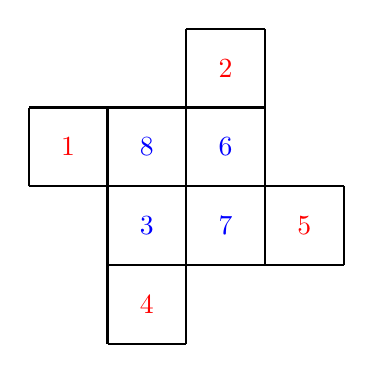
\begin{tikzpicture}
    \draw[help lines, black, thick] (0,0) grid (1,1) (1,-2) grid (2,1) (2,-1) grid (3,2) (3,-1) grid (4,0);
    \node [red] at (2.5,1.5) {$2$};
    \node [red] at (0.5,0.5) {$1$};
    \node [blue] at (1.5,0.5) {$8$};
    \node [blue] at (2.5,0.5) {$6$};
    \node [blue] at (1.5,-0.5) {$3$};
    \node [blue] at (2.5,-0.5) {$7$};
    \node [red] at (3.5,-0.5) {$5$};
    \node [red] at (1.5,-1.5) {$4$};
  \end{tikzpicture}
\end{center}

Another distinct solution may be obtained with the same middle numbers by exchanging $6$ and $3$:
\begin{center}
\subsubsection*{Solution 2: $\mathbf{S=15}$}
  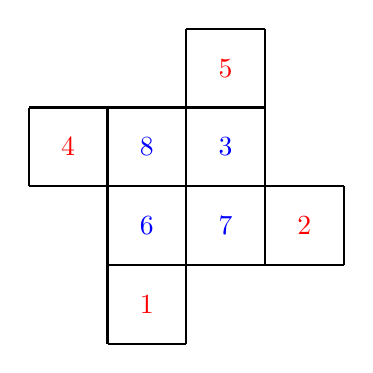
\begin{tikzpicture}
    \draw[help lines, black, thick] (0,0) grid (1,1) (1,-2) grid (2,1) (2,-1) grid (3,2) (3,-1) grid (4,0);
    \node [red] at (2.5,1.5) {$5$};
    \node [red] at (0.5,0.5) {$4$};
    \node [blue] at (1.5,0.5) {$8$};
    \node [blue] at (2.5,0.5) {$3$};
    \node [blue] at (1.5,-0.5) {$6$};
    \node [blue] at (2.5,-0.5) {$7$};
    \node [red] at (3.5,-0.5) {$2	$};
    \node [red] at (1.5,-1.5) {$1$};
  \end{tikzpicture}
\end{center}


\textbf{Consider $\mathbf{S=14~(M=20)}$}. It is clear that if $8$ and $7$ are to be in the middle, they must be along a diagonal and they must be complemented by $(3,2)$ or $(4,1)$. However, $8+2=7+3$ rules out $(8,7)$ and $(3,2)$ in the middle. The other combination does work. So a solution with $S=14$ is:
\begin{center}
\subsubsection*{Solution 3: $\mathbf{S=14}$}
  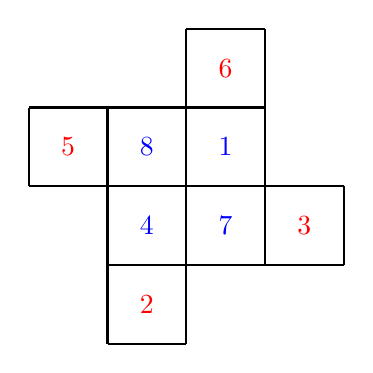
\begin{tikzpicture}
    \draw[help lines, black, thick] (0,0) grid (1,1) (1,-2) grid (2,1) (2,-1) grid (3,2) (3,-1) grid (4,0);
    \node [red] at (2.5,1.5) {$6$};
    \node [red] at (0.5,0.5) {$5$};
    \node [blue] at (1.5,0.5) {$8$};
    \node [blue] at (2.5,0.5) {$1$};
    \node [blue] at (1.5,-0.5) {$4$};
    \node [blue] at (2.5,-0.5) {$7$};
    \node [red] at (3.5,-0.5) {$3$};
    \node [red] at (1.5,-1.5) {$2$};
  \end{tikzpicture}
\end{center}

Another solution may be found with the same middle numbers by exchanging $1$ and $4$:
\begin{center}
\subsubsection*{Solution 4: $\mathbf{S=14}$}
  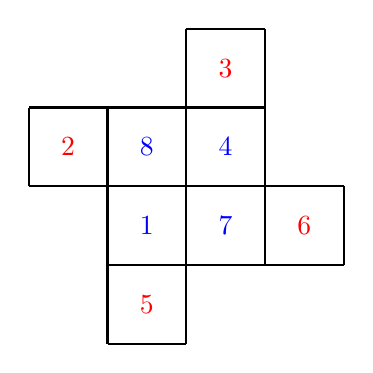
\begin{tikzpicture}
    \draw[help lines, black, thick] (0,0) grid (1,1) (1,-2) grid (2,1) (2,-1) grid (3,2) (3,-1) grid (4,0);
    \node [red] at (2.5,1.5) {$3$};
    \node [red] at (0.5,0.5) {$2$};
    \node [blue] at (1.5,0.5) {$8$};
    \node [blue] at (2.5,0.5) {$4$};
    \node [blue] at (1.5,-0.5) {$1$};
    \node [blue] at (2.5,-0.5) {$7$};
    \node [red] at (3.5,-0.5) {$6$};
    \node [red] at (1.5,-1.5) {$5$};
  \end{tikzpicture}
\end{center}

Are there other solutions for $M=20$, $S=14$? If $8$ and $6$ are in the middle, they must be along a diagonal and joined by $(5,1)$ or $(4,2)$. However, $(5,1)$ can be ruled out since $8$ and $1$ would need to be aligned with $5$ to sum to $14$. And likewise $(4,2)$ can be ruled out since $8$ and $2$ would need to be aligned with $4$ to sum to $14$. Now, if $8$ and $5$ are in the middle, it would have to be with $(4,3)$. But $8$ and $3$ must be on a diagonal since they sum to $11$ and if they were aligned would require another $3$ to sum to $14$, which is not allowed. 

\begin{center}
\subsubsection*{Solution 5: $\mathbf{S=14}$}
  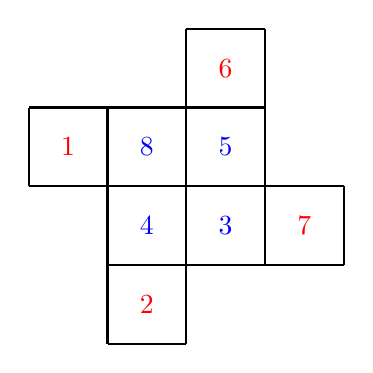
\begin{tikzpicture}
    \draw[help lines, black, thick] (0,0) grid (1,1) (1,-2) grid (2,1) (2,-1) grid (3,2) (3,-1) grid (4,0);
    \node [red] at (2.5,1.5) {$6$};
    \node [red] at (0.5,0.5) {$1$};
    \node [blue] at (1.5,0.5) {$8$};
    \node [blue] at (2.5,0.5) {$5$};
    \node [blue] at (1.5,-0.5) {$4$};
    \node [blue] at (2.5,-0.5) {$3$};
    \node [red] at (3.5,-0.5) {$7$};
    \node [red] at (1.5,-1.5) {$2$};
  \end{tikzpicture}
\end{center}

Another distinct solution may be obtained with the same middle numbers by exchanging $5$ and $4$:
\begin{center}
\subsubsection*{Solution 6: $\mathbf{S=14}$}
  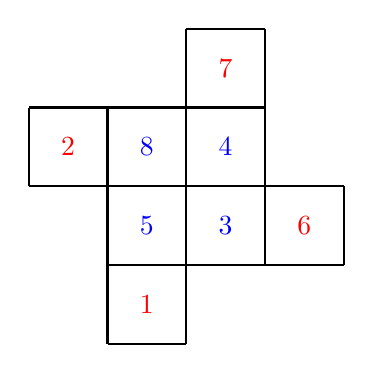
\begin{tikzpicture}
    \draw[help lines, black, thick] (0,0) grid (1,1) (1,-2) grid (2,1) (2,-1) grid (3,2) (3,-1) grid (4,0);
    \node [red] at (2.5,1.5) {$7$};
    \node [red] at (0.5,0.5) {$2$};
    \node [blue] at (1.5,0.5) {$8$};
    \node [blue] at (2.5,0.5) {$4$};
    \node [blue] at (1.5,-0.5) {$5$};
    \node [blue] at (2.5,-0.5) {$3$};
    \node [red] at (3.5,-0.5) {$6$};
    \node [red] at (1.5,-1.5) {$1$};
  \end{tikzpicture}
\end{center}

Now if $7$ and $6$ are in the middle, it would have to be with $4$ and $3$. But since $7+3=6+4$, $7$ and $6$ would have to be arranged on the same row or column. But that won't work since $4+3=7$ and another $7$ cannot be used. We do not need to look further down since $6+5=11>10=M/2$, implying that if we place $6$ and $5$ in the middle, we cannot reach the sum $M=20$ with smaller numbers like $4$, $3$. 

\textbf{Consider $\mathbf{S=13~(M=16)}$}. There are two ways to arrange $(8,5,2,1)$ in the middle.
\begin{center}
\subsubsection*{Solution 7: $\mathbf{S=13}$}
  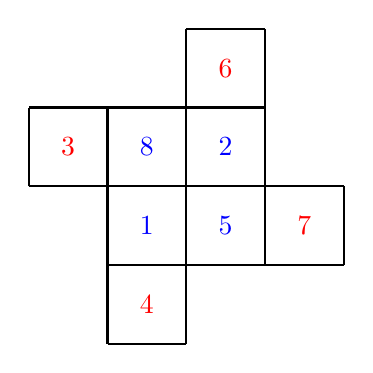
\begin{tikzpicture}
    \draw[help lines, black, thick] (0,0) grid (1,1) (1,-2) grid (2,1) (2,-1) grid (3,2) (3,-1) grid (4,0);
    \node [red] at (2.5,1.5) {$6$};
    \node [red] at (0.5,0.5) {$3$};
    \node [blue] at (1.5,0.5) {$8$};
    \node [blue] at (2.5,0.5) {$2$};
    \node [blue] at (1.5,-0.5) {$1$};
    \node [blue] at (2.5,-0.5) {$5$};
    \node [red] at (3.5,-0.5) {$7$};
    \node [red] at (1.5,-1.5) {$4$};
  \end{tikzpicture}
\end{center}

Another distinct solution may be obtained with the same middle numbers by exchanging $1$ and $2$:
\begin{center}
\subsubsection*{Solution 8: $\mathbf{S=13}$}
  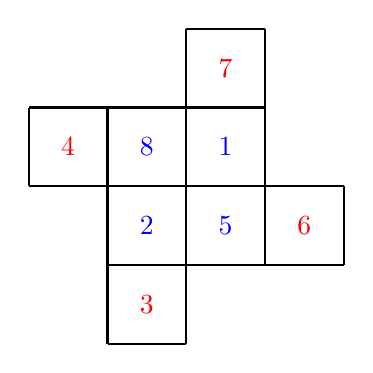
\begin{tikzpicture}
    \draw[help lines, black, thick] (0,0) grid (1,1) (1,-2) grid (2,1) (2,-1) grid (3,2) (3,-1) grid (4,0);
    \node [red] at (2.5,1.5) {$7$};
    \node [red] at (0.5,0.5) {$4$};
    \node [blue] at (1.5,0.5) {$8$};
    \node [blue] at (2.5,0.5) {$1$};
    \node [blue] at (1.5,-0.5) {$2$};
    \node [blue] at (2.5,-0.5) {$5$};
    \node [red] at (3.5,-0.5) {$6$};
    \node [red] at (1.5,-1.5) {$3$};
  \end{tikzpicture}
\end{center}


Likewise, there are two ways to arrange $6,5,4,1$ in the middle. 
\begin{center}
\subsubsection*{Solution 9: $\mathbf{S=13}$}
  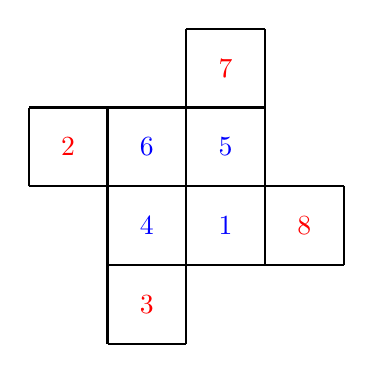
\begin{tikzpicture}
    \draw[help lines, black, thick] (0,0) grid (1,1) (1,-2) grid (2,1) (2,-1) grid (3,2) (3,-1) grid (4,0);
    \node [red] at (2.5,1.5) {$7$};
    \node [red] at (0.5,0.5) {$2$};
    \node [blue] at (1.5,0.5) {$6$};
    \node [blue] at (2.5,0.5) {$5$};
    \node [blue] at (1.5,-0.5) {$4$};
    \node [blue] at (2.5,-0.5) {$1$};
    \node [red] at (3.5,-0.5) {$8$};
    \node [red] at (1.5,-1.5) {$3$};
  \end{tikzpicture}
\end{center}

Another solution may be found with the same middle numbers by exchanging $5$ and $4$:
\begin{center}
\subsubsection*{Solution 10: $\mathbf{S=13}$}
  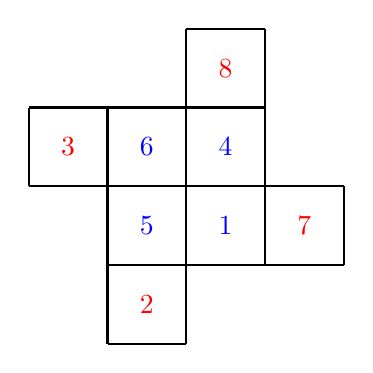
\begin{tikzpicture}
    \draw[help lines, black, thick] (0,0) grid (1,1) (1,-2) grid (2,1) (2,-1) grid (3,2) (3,-1) grid (4,0);
    \node [red] at (2.5,1.5) {$8$};
    \node [red] at (0.5,0.5) {$3$};
    \node [blue] at (1.5,0.5) {$6$};
    \node [blue] at (2.5,0.5) {$4$};
    \node [blue] at (1.5,-0.5) {$5$};
    \node [blue] at (2.5,-0.5) {$1$};
    \node [red] at (3.5,-0.5) {$7$};
    \node [red] at (1.5,-1.5) {$2$};
  \end{tikzpicture}
\end{center}

\textbf{Consider $\mathbf{S=12~(M=12)}$}. These sums are small. Because $1+2+3=6$, candidates for the middle are $(6,3,2,1)$ and $(5,4,2,1)$ only. We can have $(6,1)$ and $(6,2)$ on the same row, but clearly not $(6,3)$. We must therefore have $6$ and $3$ on a diagonal: 
\begin{center}
\subsubsection*{Solution 11: $\mathbf{S=12}$}
  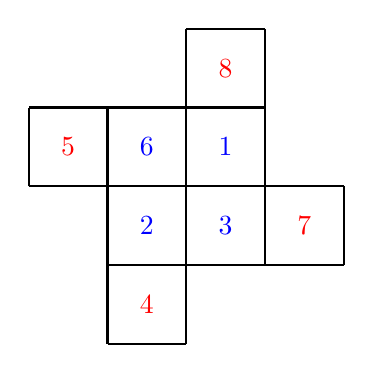
\begin{tikzpicture}
    \draw[help lines, black, thick] (0,0) grid (1,1) (1,-2) grid (2,1) (2,-1) grid (3,2) (3,-1) grid (4,0);
    \node [red] at (2.5,1.5) {$8$};
    \node [red] at (0.5,0.5) {$5$};
    \node [blue] at (1.5,0.5) {$6$};
    \node [blue] at (2.5,0.5) {$1$};
    \node [blue] at (1.5,-0.5) {$2$};
    \node [blue] at (2.5,-0.5) {$3$};
    \node [red] at (3.5,-0.5) {$7$};
    \node [red] at (1.5,-1.5) {$4$};
  \end{tikzpicture}
\end{center}

Another solution may be found with the same middle numbers by exchanging $1$ and $2$:
\begin{center}
\subsubsection*{Solution 12: $\mathbf{S=12}$}
  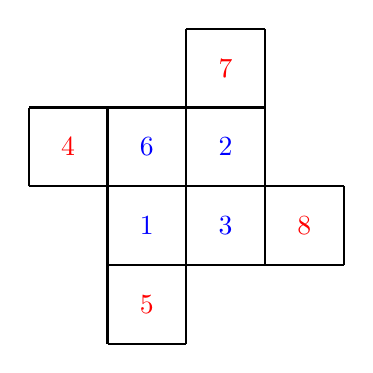
\begin{tikzpicture}
    \draw[help lines, black, thick] (0,0) grid (1,1) (1,-2) grid (2,1) (2,-1) grid (3,2) (3,-1) grid (4,0);
    \node [red] at (2.5,1.5) {$7$};
    \node [red] at (0.5,0.5) {$4$};
    \node [blue] at (1.5,0.5) {$6$};
    \node [blue] at (2.5,0.5) {$2$};
    \node [blue] at (1.5,-0.5) {$1$};
    \node [blue] at (2.5,-0.5) {$3$};
    \node [red] at (3.5,-0.5) {$8$};
    \node [red] at (1.5,-1.5) {$5$};
  \end{tikzpicture}
\end{center}

To sum up, there are $12$ solutions. We have $2$ solutions that sum to $12$ and $2$ solutions that sum to $15$. And we have $4$ solutions that sum to $13$ and $4$ solutions that sum to $14$. The solutions come in pairs, reflecting the existence of a fundamental symmetry not captured by a simple rotation. If we consider only the solutions characterized by a unique combination of middle numbers, there are $6$ such solutions only. 

The six ``fundamental solutions'' are: For $S=12$: $(1,2,3,6)$. For $S=13$: $(1,4,5,6)$ and $(1,2,5,8)$. For $S=14$: $(3,4,5,8)$ and $(1,4,7,8)$. For $S=15$: $(3,6,7,8)$. 

\end{document}
